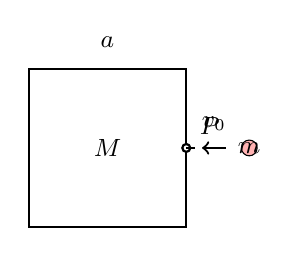
\begin{tikzpicture}[scale=1, font=\small]
  % Problem 5-6: Square frame with hole P, ball approaching
  % Square frame
  \draw[thick] (-1, 0) -- (-1, 2) -- (1, 2) -- (1, 0) -- cycle;

  % Small hole P at right side midpoint
  \draw[thick, fill=white] (1, 1) circle (0.05);
  \node[above right] at (1.05, 1.05) {$P$};

  % Ball approaching from right
  \filldraw[fill=red!30] (1.8, 1) circle (0.1);
  \node at (1.8, 1) {$m$};

  % Velocity arrow
  \draw[->, thick] (1.5, 1) -- (1.2, 1);
  \node[above] at (1.35, 1.1) {$\pmb{v}_0$};

  % Angle indication
  \draw[dashed] (1, 1) -- (1.5, 1);

  % Square label
  \node at (0, 1) {$M$};
  \node[above] at (0, 2.15) {$a$};
  \node[right] at (1.05, 1) {};
\end{tikzpicture}
